\documentclass[10pt]{amsart}
\usepackage{amsmath, amssymb, amsthm,graphicx}
\usepackage[font=small,labelfont=md,textfont=it]{caption}
\usepackage{floatrow,float}
\usepackage[titletoc, title]{appendix}
\usepackage[colorlinks,linkcolor=blue,citecolor=blue]{hyperref}
\usepackage[hyperpageref]{backref}
\usepackage{longtable}
\usepackage{pgfplots}
\pgfplotsset{compat=1.18}
\usepackage{diagbox}
\usepackage{booktabs,makecell,multirow}
\usepackage[capitalise, nosort]{cleveref}
\usepackage{cases,color}
\usepackage{algorithm}
\usepackage{algorithmic}
\usepackage{amsmath,bm}
%\usepackage{geometry}

\usepackage{tcolorbox}
\usepackage{array}
\renewcommand\arraystretch{1.5}

\newtheorem{algo}{Algorithm}
%\geometry{left = 3cm,right=3cm,top =3cm,bottom = 3.5cm }

\DeclareMathOperator{\D}{D}
\DeclareMathOperator{\I}{I}

\crefname{equation}{}{}
\crefname{lem}{Lemma}{Lemmas}
\crefname{thm}{Theorem}{Theorems}

\newcommand{\dd}{\,{\rm d}}
\newcommand{\R}{\,{\mathbb R}}
\newcommand{\bs}{\boldsymbol}
\newcommand{\dual}[1]{\left\langle {#1} \right\rangle}
\newcommand{\proxi}[0]{ {\bf prox}}
\newcommand{\J}[0]{ {\bf J}}
\newcommand{\dom}[0]{ {\bf dom\,}}
\newcommand{\argmin}[0]{ {\mathrm {argmin}\,}}
\newcommand{\inner}[1]{\left({#1} \right)}
\newcommand{\jmp}[1]{{[\![ {#1} ]\!]}}
\newcommand{\nm}[1]{\left\lVert {#1} \right\rVert}
\newcommand{\snm}[1]{\left\lvert {#1} \right\rvert}
\newcommand{\ssnm}[1]
{
  \left\vert\kern-0.25ex
  \left\vert\kern-0.25ex
  \left\vert
  {#1}
  \right\vert\kern-0.25ex
  \right\vert\kern-0.25ex
  \right\vert
}
\newcommand{\lsnm}[1]{\snm{#1}^{\text{\tiny L}}}
\newcommand{\rsnm}[1]{\snm{#1}^{\text{\tiny R}}}

\renewcommand{\algorithmicrequire}{ \textbf{Input:}} %Use Input in the format of Algorithm
\renewcommand{\algorithmicensure}{ \textbf{Output:}} %UseOutput in the format of Algorithm

\makeatletter
\def\spher@harm#1{%
  \vbox{\hbox{%
    \offinterlineskip
    \valign{&\hb@xt@2\p@{\hss$##$\hss}\vskip.2ex\cr#1\crcr}%
  }\vskip-.36ex}%
}
\def\gshone{\spher@harm{.}}
\def\gshtwo{\spher@harm{.&.}}
\def\gshthree{\spher@harm{.&.&.}}
\let\gsh\spher@harm
\makeatother

\newtheorem{theorem}{Theorem}[section]
\newtheorem{lemma}[theorem]{Lemma}
\newtheorem{corollary}[theorem]{Corollary}
\newtheorem{proposition}[theorem]{Proposition}
\newtheorem{definition}[theorem]{Definition}
\newtheorem{example}[theorem]{Example}
\newtheorem{exercise}[theorem]{Exercise}
\newtheorem{question}[theorem]{Question}
\newtheorem{remark}[theorem]{Remark}
\newtheorem{alg}[theorem]{Algorithm}

%\newtheorem{algor}{Algorithm}
% \newtheorem{alg}{algorithm}
% %\newtheorem{alg}[theorem]{Algorithm}
% \newtheorem{coro}{corollary}[section]
% \newtheorem{prop}{proposition}[section]
% \newtheorem{Def}{definition}[section]
% \newtheorem{assum}{assumption}
% \newtheorem{lem}{lemma}[section]
% \newtheorem{rem}{remark}[section]
% \newtheorem{thm}{theorem}[section]
% \newtheorem{example}{example}[section]
% \newtheorem{exercise}{exercise}

\newcommand{\LH}[1]{\textcolor{blue}{#1}}
\newcommand{\LC}[1]{\textcolor{red}{#1}}
\newcommand{\JW}[1]{\textcolor{cyan}{#1}}
  \newcounter{mnote}
\setcounter{mnote}{0}
\newcommand{\mnote}[1]{\addtocounter{mnote}{1}
	\ensuremath{{}^{\bullet\arabic{mnote}}}
	\marginpar{\footnotesize\em\color{red}\ensuremath{\bullet\arabic{mnote}}#1}}
\let\oldmarginpar\marginpar
\renewcommand\marginpar[1]{\-\oldmarginpar[\raggedleft\footnotesize #1]%
	{\raggedright\footnotesize #1}}

%\renewcommand\qedsymbol{\hfill\ensuremath{\blacksquare}}

\makeatletter\def\@captype{table}\makeatother
%\newcommand{\nm}[1]{\left\lVert {#1} \right\rVert}
%\newcommand{\proxi}[0]{ {\bf prox}}
\newcommand{\gf}{\nabla f}

\begin{document}
\title{Stochastic Gradient Langevin Dynamics for Bayesian Learning}
\author{Zeyi Xu}\date{\today}
\begin{abstract}
Stochastic Gradient Langevin Dynamics (SGLD) is a sampling method proposed in the paper \textit{Bayesian Learning via Stochastic Gradient Langevin Dynamics} \cite{10.5555/3104482.3104568}. It stands at the intersection of stochastic optimization and Langevin-proposed MCMC methods. In this report, we summarize the mathematical foundations of the method, implement the method and test its performance on various learning tasks.
\end{abstract}
\maketitle

\tableofcontents
\section{Introduction}
The main points of the report are listed as follows:
\begin{itemize}
    \item The paper considers the Bayesian learning problem, that is, given probability model, do the Maximum A Posterior estimate from sample data.
    \item In the paper, the authors focus on the Bayesian modeling with parametric models.
    \item The authors derived the SGLD algorithm by combining Stochastic gradient method with Langevin dynamics.
    \item In essence, the problem is about sampling from a known distribution. Besides all the standard MCMC methods, Hamiltonian Monte Carlo (HMC) is of interest as an accelerating sampling method. \cite{chen2014stochasticgradienthamiltonianmonte} develops a way to incorporate stochastic gradient into HMC method. Recent years, generative models have caught wide attention for their expressive power and scaling property \cite{Bond_Taylor_2022}.
    \item In this report, we used SGLD to solve 2 Bayesian learning problems. One is the linear regression problem, the other one is the logistic regression problem.
\end{itemize}
The rest of the report is organized as follows. In section 2, we briefly go over the problem setting, and elaborate the method as a combination of stochastic gradient method and Langevin dynamics. In section 3, we implement the method and report the results of numerical experiments.

\section{Method}
We consider the $n$-dimensional Bayesian learning problem with a large scale dataset. Let $\theta\in\mathbb{R}^n$ be a set of model parameters, $\{x_i\}_{i=1}^N$ data points. The problem is to compute the MAP estimation 
\begin{equation}
    p(\theta|x)\propto p(\theta)\prod_{i=1}^N p(x_i|\theta)
\end{equation}
using prior distribution $p(\cdot)$ and likelihood function $p(x|\theta)$.
Equivalently, maximize the logarithm of posterior distribution density
\begin{equation} \label{logmap}
    \max_{\theta} f(\theta):=\log p(\theta) + \sum_{i=1}^N \log p(x_i|\theta).
\end{equation}
For this optimization problem, a classic method is to do gradient ascent,
\begin{equation}
    \theta_{k+1}=\theta_k + \alpha_k \gf(\theta_k).
\end{equation}
The drawback of this method is that the model replies deterministically on the training data $\{x_i\}$, and it might overfit and could not generalize to new data. To circumvent this situation, consider adding a stochastic term into the update
\begin{equation}\label{langevin_discrete}
    \theta_{k+1}=\theta_k + \alpha_k \gf(\theta_k) + \sqrt{2\alpha_k}\xi_k,
\end{equation}
where $\xi_k\sim N(0,I_n)$ is a $n$-dimensional standard normal vector. It can be seen as the $\alpha_k$-discretization of the following Langevin-dynamics
\begin{equation} \label{langevin}
    d\theta_t = -\nabla U(\theta_t)dt+\sqrt{2}dB_t,
\end{equation}
where $U$ is the potential, $U(\theta)=-f(\theta)$. In continuous-time dynamics, \eqref{langevin} converges to its stationary distribution 
\begin{equation}
    \pi(\theta)\propto e^{-U(\theta)}.
\end{equation}
In discrete time, such property will not naturally hold, but it can be fit into the framework of Rosenbluth-Hastings by adding a probability of acceptance, making it a typical MCMC algorithm with the proposal in the form of \eqref{langevin_discrete}. This is called the Metropolis adjusted Langevin algorithm (MALA). 

Though provably faster than the na\"ive proposals such as Gaussian, MALA needs to evaluate the gradients of all current sample points each step. This becomes computationally expensive when (1) the sample size is extremely large (2) the gradient is hard to evaluate.

Stochastic Gradient provides a way to overcome this issue. Instead of evaluating the full gradient, it only computes gradients for a mini-batch of samples $\{x_{ki}\}_{i=1}^m$, and replace the gradient term by the partial gradient on these points. Combining it with \eqref{logmap}, \eqref{langevin_discrete}, we get the so-called Stoachastic Gradient Langevin Dynamics 
\begin{equation}\label{SGLD}
    \theta_{k+1}=\theta_k + \alpha_k\left[\log p(\theta_k)+\frac{N}{n}\sum_{i=1}^n \log p(x_{ki}|\theta_k)\right]+\sqrt{2\alpha_k}\xi_k    
\end{equation}
where $\xi_k\sim N(0,I_n)$.

\section{Numerical Experiments}
In this section, we perform 2 numerical experiments to validify SGLD in Bayesian learning tasks. All the necessary code for this section can be found at GitHub repository \href{https://github.com/ZeyiXuu/SGLD.git}{https://github.com/ZeyiXuu/SGLD.git}. As the original paper does not come with code, the code above is adapted from the existing third-party code on SGLD: \href{https://github.com/LouisBouvier/BML_Stochastic_Langevin_Dynamics.git}{https://github.com/LouisBouvier/BML\_Stochastic\_Langevin\_Dynamics.git} and \href{https://github.com/JavierAntoran/Bayesian-Neural-Networks.git}{https://github.com/JavierAntoran/Bayesian-Neural-Networks.git}.
\subsection{Bayesian Linear Regression using SGLD}

In this experiment, we apply Stochastic Gradient Langevin Dynamics to perform Bayesian Linear Regression with a Laplace prior of scale \( b=1 \). For now, we fix the variance of the Gaussian likelihood to \( \sigma^2=1 \). We also compare Stochastic Gradient Langevin Dynamics to other sampling methods to test its efficiency, particularly its speed.

The model is as follows:
\[
p(\beta) \sim \mathcal{L}(0, 1), \quad \text{i.e.} \quad p(\beta) \propto \exp(-\|\beta\|_1),
\]
For all \( i \in \{1, \dots, N\} \), 
\[
y_i \sim \mathcal{N}(x_i^{\top}\beta, \sigma^2), \quad \text{i.i.d.}
\]
Thus, the log posterior is:
\[
\log p(\beta | X, y) \propto - \sum_{i=1}^N (x_i^{\top}\beta - y_i)^2 - \|\beta \|_1 = - \|X\, \beta - y\|_2^2 - \|\beta \|_1
\]
Using the fact that a subgradient of the log-prior is \( \partial_{\beta} \log p(\beta) = - \mathrm{sign}(\beta) \) and letting \( X \) represent the data matrix, i.e.
\[
X = \begin{pmatrix}
x_1\\
\vdots\\
x_n
\end{pmatrix} \in \mathbb{R}^{n \times d}
\]
and \( y \) the vector of labels, we can write a subgradient of the log-posterior as:
\[
\partial_{\beta} \log p(\beta | X, y) = - X^{\top}X \, \beta + X^{\top}y - \mathrm{sign}(\beta).
\]

To test validity of the SGLD method, We apply it to synthetic data. Let $y=0.02x^3+x^2+0.3x$ be the objective relation. Let $x$ be $250$ points randomly chosen from $[-5,5]$, and corresponding $y$ be computed from the desired relation. Apply Mini Batch SGLD method with $\texttt{batch\_size}=5$ for $5000$ iterations. The resulting parameters form a well-trained linear regression model. Use the model to do prediction, the results are quite close to the ground truth (Fig. \ref{fig:lr}).
\begin{figure}[ht]
    \centering
    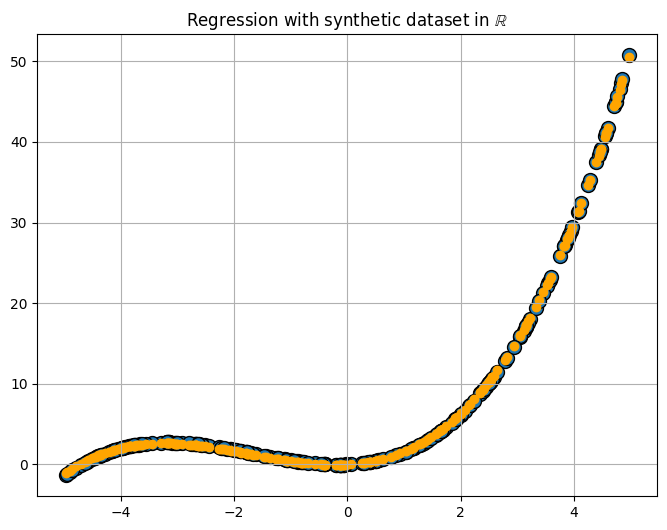
\includegraphics[width=0.5\linewidth]{graph/SGLD_LR.png}
    \caption{The performance of SGLD on linear regression tasks}
    \label{fig:lr}
\end{figure}

\subsection{Bayesian Logistic Regression using SGLD}
In this experiment, we apply Stochastic Gradient Langevin Dynamics to perform Bayesian Linear Regression with a Laplace prior of scale \( b=1 \). Notice that, in this problem, the log posterior becomes:
$$
\log p(\beta | X, y) \propto \sum_{i=1}^N \log \sigma(y_i \cdot \beta^{\top}x_i) - \|\beta\|_1
$$
where $\sigma$ is the sigmoid function: $\sigma(x)=\frac{1}{1+\exp(-z)}$. We can then write a subgradient of the log-posterior using the fact that $\forall z \in \mathbb{R}, \sigma'(z) = (1 - \sigma(z)) \cdot \sigma(z)$, and the subgradient of the log-prior is $\partial_{\beta} \log p(\beta) = - \text{sign}(\beta)$:
$$
\partial_{\beta} \log p(\beta | X, y) = \sum_{i=1}^N y_i \cdot x_i \left( 1 - \sigma(y_i \cdot \beta^{\top}x_i) \right) - \text{sign}(\beta)
$$
To test validity of the SGLD method, We apply it to synthetic data. We generate two clusters containing $1500$ sample points centered respectively at $(-2,2)$ and $(2,-2)$ with $\texttt{std}=1.3$. Apply Mini Batch SGLD method with $\texttt{batch\_size}=5$ for $5000$ iterations. The resulting parameters form a well-trained Logistic regression model. Use the model to do prediction, we gained a high accuracy for point separation (Fig. \ref{fig:logr}(a)). Fig \ref{fig:logr}(b) is the contour map of the predicted probability given by the regression model. When a point deviates from the straight line $y=-x$, its predicted value will rise or drop quickly to $1$ or $0$, showing that the model will give it a clear and correct classification.
\begin{figure}[ht]
    \centering
    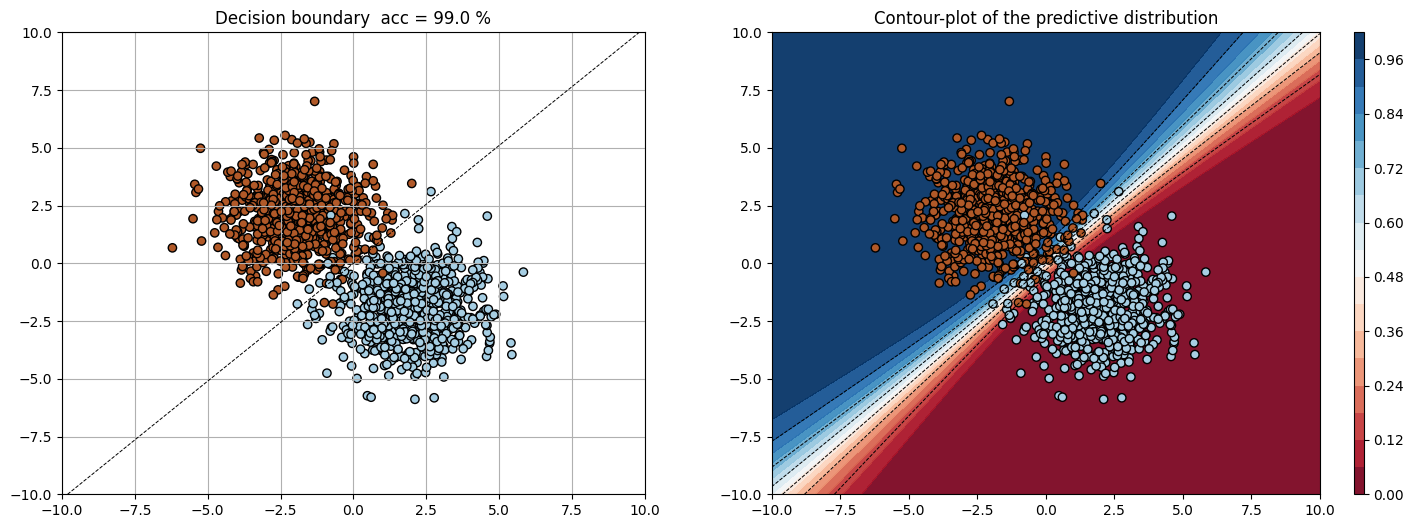
\includegraphics[width=1\linewidth]{graph/SGLD_LogR.png}
    \caption{Classification results of the Bayesian Logistic Regression model}
    \label{fig:logr}
\end{figure}

\section{Conclusion}
In this project, we summarize the mathematical aspects of the Stochastic Gradient Langevin Dynamics (SGLD) as a combination of Stochastic Gradient Descent with Langevin Dynamics. We implement the algorithm and test it on simple regression tasks with synthetic data. The results show the validity of this method. Future directions of this project are:
\begin{itemize}
    \item[(1)] comparing the efficiency of SGLD with other more naive sampling methods;
    \item[(2)] recognizing the accelerated methods to SGLD, such as SAGA-LD and SVRG-LD, and developing more efficient Bayesian learning methods;
    \item[(3)] using acclerated optimization methods from math community to further accelerate Langevin-based sampling methods.
\end{itemize}

\bibliographystyle{abbrv}
\bibliography{reference}
\end{document}